\documentclass[12pt,a4paper]{report}

% --- Paquetes de Idioma y Codificación ---
\usepackage[utf8]{inputenc}
\usepackage[T1]{fontenc}
\usepackage[spanish, es-tabla]{babel}

% --- Diseño de Página ---
\usepackage{geometry}
\geometry{top=2.5cm, bottom=2.5cm, left=3cm, right=3cm}

% --- Matemáticas y Símbolos ---
\usepackage{amsmath, amssymb, amsthm}

% --- Colores y Cajas ---
\usepackage[dvipsnames]{xcolor}
\usepackage[most]{tcolorbox}

% Caption

\usepackage{caption}

% Gráficos

\usepackage{graphicx}

% Espaciadora

\newcommand{\esp}{\vspace{0.5cm}}

% promedio

\newcommand{\prom}[1]{\left\langle #1 \right\rangle}

% ket

\newcommand{\ket}[1]{| #1 \rangle}

% bra

\newcommand{\bra}[1]{\langle #1 |}

% braket

\newcommand{\braket}[2]{\langle #1 | #2 \rangle}

% Bibliografía

\usepackage[style=apa, backend=biber]{biblatex} % Estilo APA
\addbibresource{biblio.bib} % Nombre de tu archivo .bib

% Configuración de cajas personalizadas
\newtcolorbox{importante}{
	colback=red!5!white,
	colframe=red!75!black,
	title=Importante,
	fonttitle=\bfseries
}

\newtcolorbox{nota}{
	colback=blue!5!white,
	colframe=blue!75!black,
	title=Nota,
	fonttitle=\bfseries
}

% Definición de la caja de bibliografía
\newtcolorbox{bibliografia}{
	colback=gray!5!white,
	colframe=gray!75!black,
	title=Bibliografías útiles,
	fonttitle=\bfseries,
	breakable
}

% Socrative para óptica 2

\newtcolorbox{Socrative}{
	colback=orange!5!white,
	colframe=orange!75!black,
	title=Socrative,
	fonttitle=\bfseries,
	breakable
}

% Float

\usepackage{float}

% --- Hipervínculos ---
\usepackage{hyperref}
\hypersetup{
	colorlinks=true,
	linkcolor=blue,
	filecolor=magenta,      
	urlcolor=cyan,
}

% --- Datos del Documento ---
\title{Óptica II}
\author{Chengyu Jin}
\date{\today}

\begin{document}
	
	\maketitle
	
	\tableofcontents
	\newpage
	
	\chapter{Láser y LED. Principales aplicaciones}
	
	Dedicaremos este tema a dos tipos de fuentes de luz que han sido fundamentales en el desarrollo de la Óptica: el LED y el láser. La emisión del diodo emisor de luz (\textit{Light Emitting Diode}) o LED se basa en la interacción fotón electrón en semiconductores dopados, que forman uniones p-n. El primer LED fue desarrollado en torno a la misma fecha que el láser de Maiman, en 1961, por Biard y Pittman. Emitía en infrarrojo, así que no tuvo mucha aplicación práctica hasta que, en el año siguiente, Nick Holonyak desarrolló el primer LED visible (rojo). A partir de entonces, en los siguientes 20-30 años se estuvo experimentando mucho sobre materiales semiconductores para conseguir una mayor emisión y variedad de longitudes de onda, y en 1994 se produce el primer \textit{Super bright LED}, inventado por Shuji Nakamura. Desde entonces, la tecnología LED ha avanzado tanto que ha sido capaz de convertirse en la fuente de iluminación dominante en espacios interiores, y avanza fuerte también en el campo de la iluminación nocturna en espacios urbanos.
	
	\esp
	
	Láser es un acrónimo de \textit{Light Amplification by stimulated emission of radiation}. Ha supuesto una verdadera revolución en la ciencia y la tecnología de los últimos 60 años. En este tema, vamos a ver brevemente algunas bases de su funcionamiento y sus características más destacadas. Pero antes, hagamos un poco de historia. La emisión láser se basa en una forma especial de interacción luz-materia que puso de manifiesto Einstein en 1916, la emisión estimulada. Pero no fue hasta 1950 que surgió la primera realización práctica de un dispositivo basado en la emisión estimulada: fue el máser, que funciona en el rango de las microondas. Fue desarrollado gracias al trabajo de C.H. Townes, A.M. Prokhorov y N.G. Basov, entre otros. En seguida, se empieza a pensar en construir un dispositivo que funcione en el rango visible. En 1958, C.H. Townes y A.L. Shawlow realizaron un estudio teórico sobre las condiciones necesarias para ello. Y en Julio de 1960, T.H. Maiman consigue el primer prototipo de láser utilizando rubí (óxido de Cromo) como medio de interacción. Las aplicaciones de ambos tipos de fuentes son muy variadas e interesantes, como veremos en los ejemplos de las secciones del tema dedicadas a los campos de aplicación. La palabra \textit{boom} seguramente se queda corta para describir la multitud de usos que tienen los láseres y fuentes de LED en la actualidad.
	
	\section{LED}
	
	En esta sección, vamos a estudiar someramente algunas de las características más relevantes de las fuentes LED, que son en definitiva un tipo de dispositivos optoelectrónicos (fuentes y detectores basados en la interacción fotón-electrón fundamentalmente en semiconductores). Nos centraremos en las fuentes en este tema, y dentro de los basados en semiconductores, veremos los LED y también los láseres de diodo en la siguiente sección. Vamos a tratar primero algunos aspectos básicos de semiconductores, para después centrarnos en el mecanismo de funcionamiento del LED y sus características de emisión, viendo algunas de las configuraciones y dispositivos más comunes y de mayor interés.
	
	\subsection{Teoría básica de semiconductores}
	
	\begin{figure}[H]
		\centering
		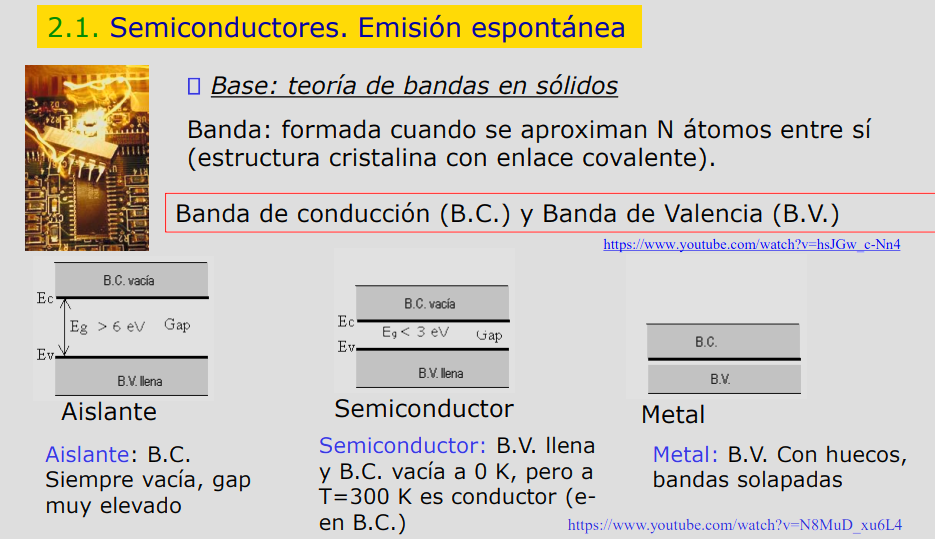
\includegraphics[width=0.7\textwidth]{IMG/led.png}
	\end{figure}
	
	\esp
	
	La base para comprender cómo funcionan los semiconductores es la teoría de bandas en sólidos. Aquí vamos a exponer de forma muy breve sólo algunos de sus aspectos más relevantes, porque es un campo muy amplio, como podrán comprobar los que tengan pensado dedicarse a la microelectrónica.
	
	\esp
	
	Los niveles de energía que pueden ocupar los electrones en átomos aislados son discretos y por lo general bastante separados (en especial los niveles inferiores de energía). Pero cuando $N$ átomos se aproximan entre sí para formar un sólido con una estructura cristalina de enlace covalente, se observa que si bien los niveles de energía de los electrones más internos no se ven afectados apreciablemente por la presencia de átomos vecinos, en cambio, los niveles energéticos más externos sufren modificaciones importantes, ya que estos electrones están siendo compartidos por varios átomos en la estructura cristalina. El acoplamiento entre las capas más externas de electrones de estos átomos da como resultado una banda de estados de energía muy próximos entre sí, en lugar de los niveles más separados propios del átomo aislado. Los niveles formados como consecuencia de este acoplamiento constituyen una banda casi continua de energía entre sus extremos inferior y superior. A la banda correspondiente a niveles de menor energía se denomina \textit{banda de valencia} (B.V.), y a la banda de niveles superiores se llama \textit{banda de conducción} (B.C.). Entre ambas bandas, queda un hueco de energía que no puede ser ocupado por los electrones, y se denomina \textit{gap} o salto.
	
	\esp
	
	La configuración de las bandas condiciona el comportamiento del material. Por ejemplo, en un aislante, la B.V. está llena y la B.C. vacía, porque el gap (mayor de 6 eV) es muy elevado y no pueden acceder los electrones a la B.C. En un metal, las bandas de conducción y valencia están solapadas, con lo que es posible siempre la movilidad de los electrones hacia la B.C. El que los electrones puedan acceder a la B.C. condiciona el que el material pueda conducir la corriente eléctrica o no. En los semiconductores, el gap es pequeño entre ambas bandas, pero no están confundidas como en los metales, con lo cual a $T = 0$K tienen la B.C. vacía, comportándose como aislantes. Pero a temperatura ambiente (300K), por agitación térmica u otros procesos, los electrones adquieren energía suficiente para saltar el gap y pasar a la B.C., con lo cual se comportan como conductores.
	
	\esp
	
	\begin{figure}[H]
		\centering
		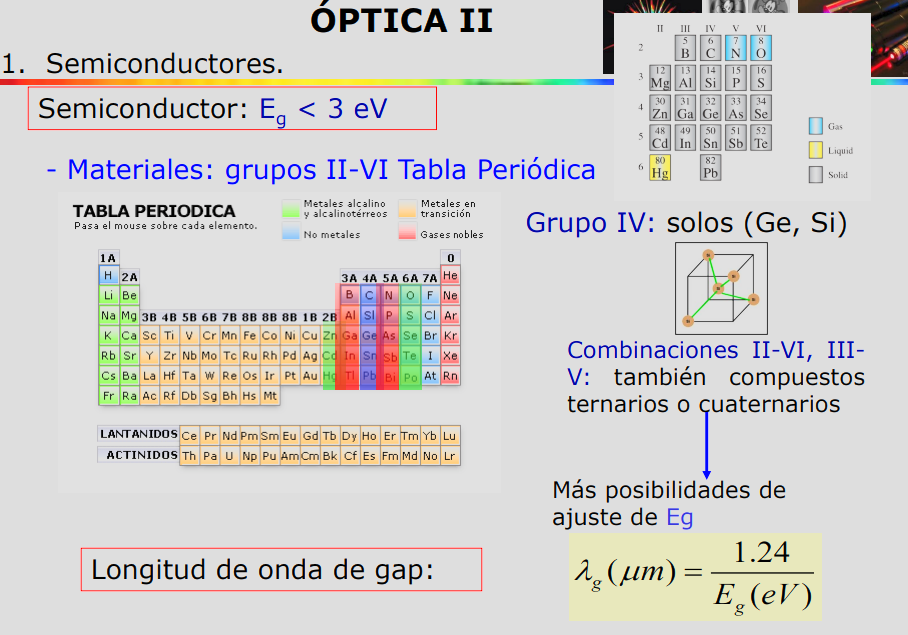
\includegraphics[width=0.7\textwidth]{IMG/led2.png}
	\end{figure}
	
	\esp
	
	Se considera que un material es semiconductor si el valor del gap no excede los $3eV$ (ver el esquema en la figura 1).
	
	\esp
	
	\begin{figure}[H]
		\centering
		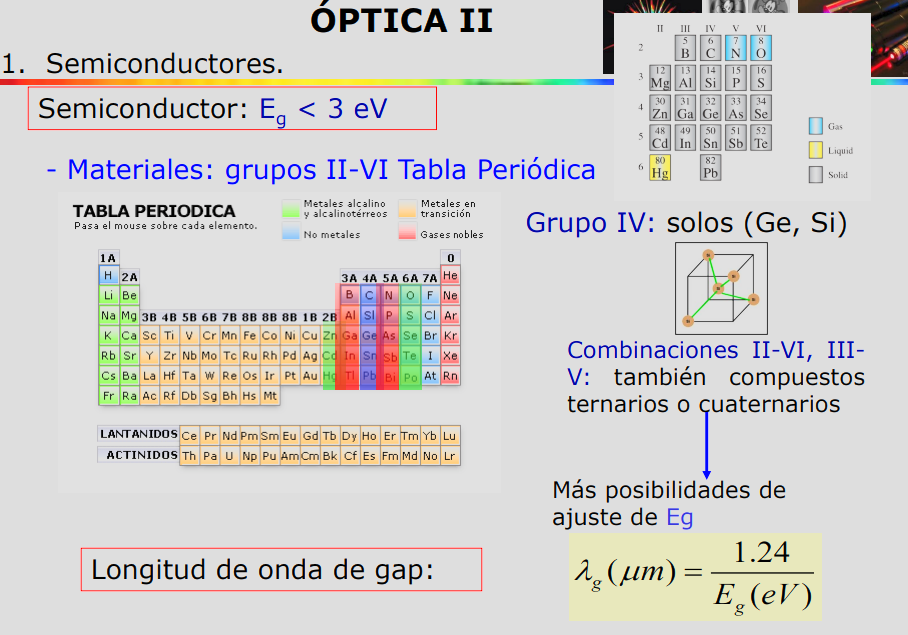
\includegraphics[width=0.7\textwidth]{IMG/led2.png}
	\end{figure}
	
	\esp
	
	Los materiales semiconductores están formados por elementos de los grupos $II$-$VI$ de la Tabla periódica. Los del grupo $IV$, como el germanio ($Ge$) o silicio ($Si$), pueden funcionar como semiconductores por sí mismos; los de los grupos $III$ y $V$, necesitan formar compuestos, igual que los de los grupos $II$ y $VI$. Los compuestos pueden ser binarios (por ejemplo, $GaAs$ o Arseniuro de Galio), ternarios ($InGaAs$) o incluso cuaternarios, lo que ofrece mayores posibilidades de ajuste para el valor de la energía de gap.
	
	\esp
	
	Los semiconductores se caracterizan, entre otros parámetros, por la longitud de onda de gap correspondiente (longitud de onda en el vacío correspondiente a la frecuencia de la transición de mínima energía entre las bandas de conducción y valencia). Se obtendría entonces considerando que la energía del gap es: $E_g = h\nu$, y a su vez, $\lambda = \frac{c}{\nu} = \frac{ch}{E_g} = \frac{1.24}{E_g}$, si expresamos $E_g$ en $eV$, y la longitud de onda quedaría entonces en micras.
	
	\esp
	
	Vamos a ver ahora brevemente cómo se produce la interacción fotón-electrón en este tipo de materiales. Hay dos procesos fundamentales: absorción de fotones para producir saltos de electrón a la B.C., con lo que se crean huecos en la B.V. (lo que se llama \textit{creación de pares electrón-hueco}), y el proceso contrario de emisión de fotones cuando un electrón pasa a ocupar un hueco de la B.V. (\textit{recombinación radiativa}). Hay que tener en cuenta que no todas las recombinaciones son radiativas. La emisión puede ser espontánea o estimulada si se dan las condiciones para ello, lo que puede dar lugar a fuentes láser basadas en semiconductores.
	
	\esp
	
	\begin{figure}[H]
		\centering
		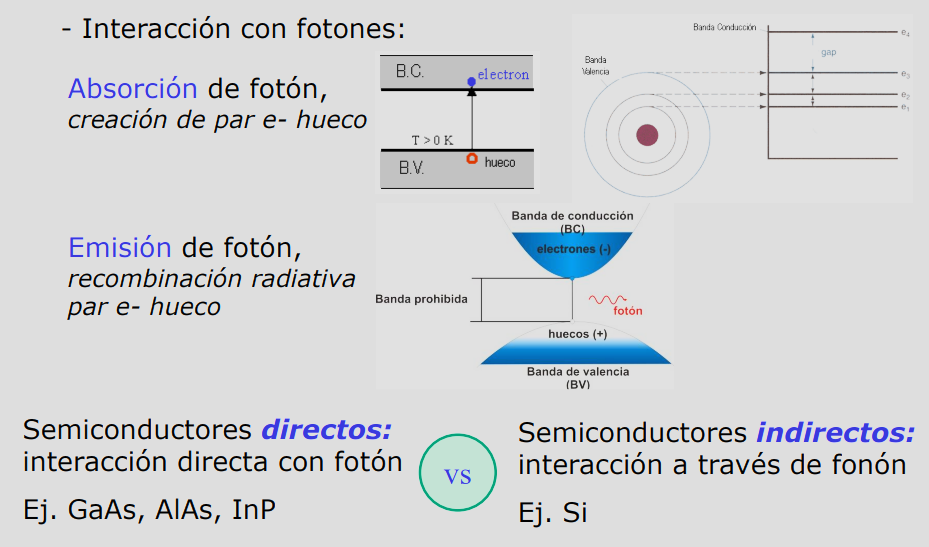
\includegraphics[width=0.7\textwidth]{IMG/led4.png}
	\end{figure}	
	
	\esp
	
	Desde el punto de vista de la interacción con los fotones, distinguimos dos tipos de semiconductores: los \textbf{directos}, en los que se dan los procesos que hemos descrito, como el $AlAs, GaAs, InP, ZnS$ y otros. Son por tanto los adecuados para constituir la base de fuentes de luz. También hay otro tipo de semiconductores en los cuales la interacción directa es con fonones (que son las partículas asociadas con el transporte de energía en ondas mecánicas y sonoras según la teoría cuántica), de forma que para que se produzca una emisión de un fotón deben convivir simultáneamente las tres partículas (electrón, fonón y fotón), con lo cual la probabilidad de recombinación radiativa es bastante menor. 
	
	\esp
	
	\begin{figure}[H]
		\centering
		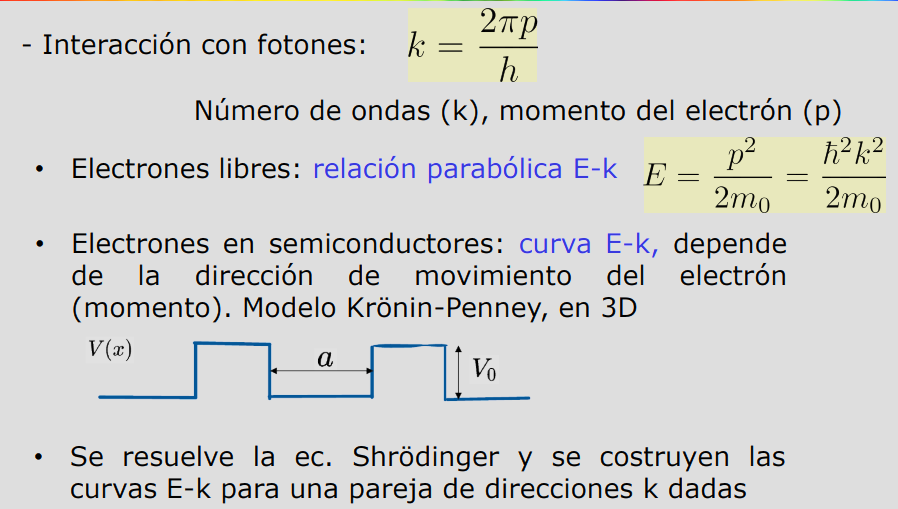
\includegraphics[width=0.7\textwidth]{IMG/led5.png}
	\end{figure}
	
	\esp
	
	Son los llamados \textbf{semiconductores indirectos}, como el $Si$. Para saber si un material es de tipo directo o indirecto, hace falta conocer su curva $E-k$ (relación energía-número de onda). El número de onda se relaciona con el momento del electrón, según $k = \frac{2\pi p}{h}$. Entonces, por ejemplo, para un electrón no ligado, la energía del electrón y el número de onda presentan una relación de tipo parabólico, ya que se cumple que:
	
	\esp
	
	\begin{equation}
		E = p^2 / 2m_0 = \hbar^2 k^2 / 2m_0
	\end{equation}
	
	\esp
	
	\begin{figure}[H]
		\centering
		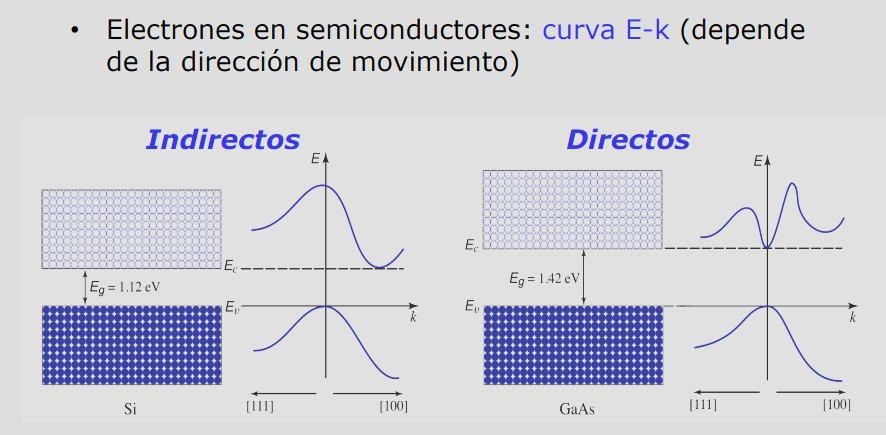
\includegraphics[width=0.7\textwidth]{IMG/led6.png}
	\end{figure}
	
	\esp
	
	En el caso de electrones (o huecos) en semiconductores, resolviendo la ecuación de Schrödinger asociada a una simplificación de la función potencial como una función periódica... se llega a que la energía es una función periódica de las tres componentes del vector $k$, que serían $(k_1, k_2, k_3)$, y las constantes de periodicidad dependen de tres variables típicas que caracterizan la estructura cristalina del compuesto. Entonces, la energía de un electrón no depende sólo del módulo de su momento, sino también de su dirección de movimiento. Esto se puede ilustrar con el diagrama $E-k$, como se muestra en la figura 2 para los casos de $GaAs$ y $Si$.
	
	\esp
	
	\begin{figure}[H]
		\centering
		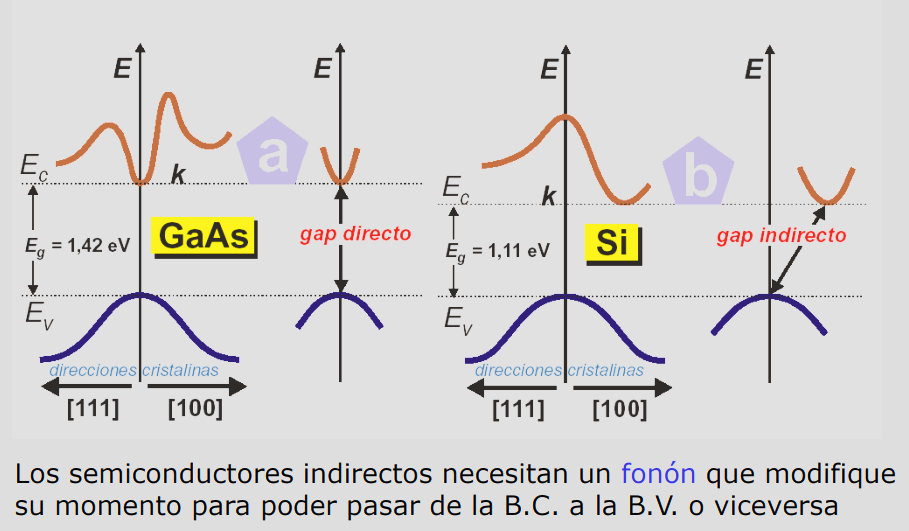
\includegraphics[width=0.7\textwidth]{IMG/led7.png}
	\end{figure}
	
	\esp
	
	Justo en la zona más alta de la banda de valencia, y en la zona más baja de la banda de conducción, las curvas $E - k$ pueden aproximarse por parábolas, y esto nos daría una \textit{masa efectiva} para los huecos y electrones respectivamente. Pero lo que más nos interesa de estas curvas es que vemos que, en el caso de los semiconductores \textit{directos}, como el $GaAs$, el valor mínimo de gap entre las bandas se da para un mismo valor de número de onda (máximo y mínimo de las curvas $E - k$ alineados), mientras que para los materiales \textit{indirectos}, como el $Si$, es necesario para el electrón cambiar su valor de momento para poder realizar la transición, porque los niveles máximo y mínimo de las dos bandas no están alineados. Por eso, los materiales indirectos necesitan de la interacción con otra partícula adicional (el \textit{fonón}) para cambiar el momento del electrón y permitir su transición a la banda de conducción, mientras que no es necesaria la intervención de los fonones en el caso de los materiales directos.
	
	\subsection{Dopaje. Uniones p-n.}
	
	\begin{figure}[H]
		\centering
		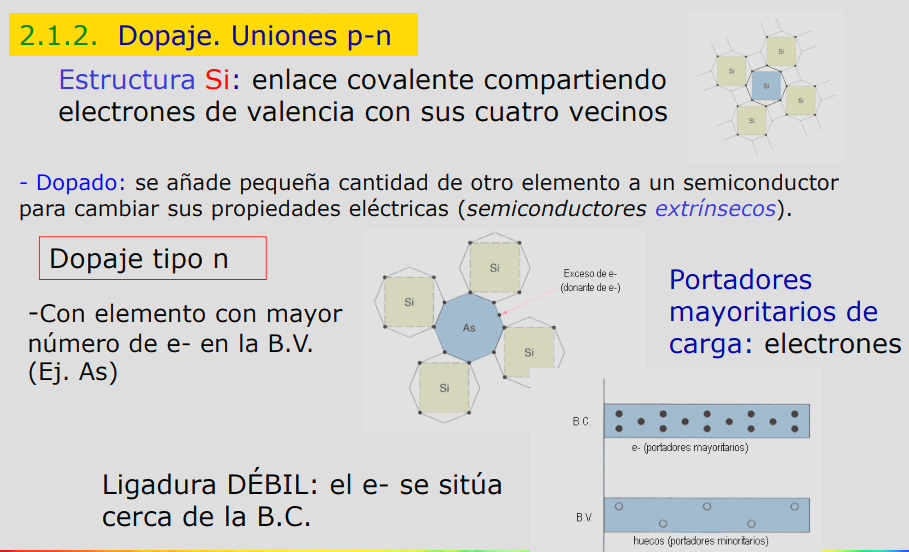
\includegraphics[width=0.7\textwidth]{IMG/led8.png}
	\end{figure}
	
	\esp
	
	En muchas ocasiones, se añade a los semiconductores una pequeña cantidad de otro elemento semiconductor, lo que permite cambiar profundamente sus propiedades ópticas y eléctricas. Este proceso se llama dopado o dopaje. Hay dos categorías principales de compuestos dopados: los \textit{tipo p} y los \textit{tipo n}. Para entender su estructura, vamos a tomar como ejemplo el $Si$, del grupo $IV$ y por tanto con cuatro electrones en su B.V. En estado puro, el $Si$ comparte estos electrones con otros átomos de $Si$ situados a su alrededor.
	
	\esp
	
	En los compuestos dopados \textit{tipo n}, cambiamos algunos átomos de $Si$ en la red por otros de un elemento con mayor número de electrones de valencia, como el $As$ que tiene cinco (pertenece al grupo $V$). Entonces, si cada átomo de $As$ comparte cuatro electrones con cuatro átomos de $Si$ vecinos, le queda un electrón sin compartir, débilmente ligado. Por lo tanto, el compuesto es un potencial donante de electrones. Estos electrones débilmente ligados se sitúan cerca de la B.C. del material, y constituyen los portadores mayoritarios de carga del compuesto.
	
	\esp
	
	\begin{figure}[H]
		\centering
		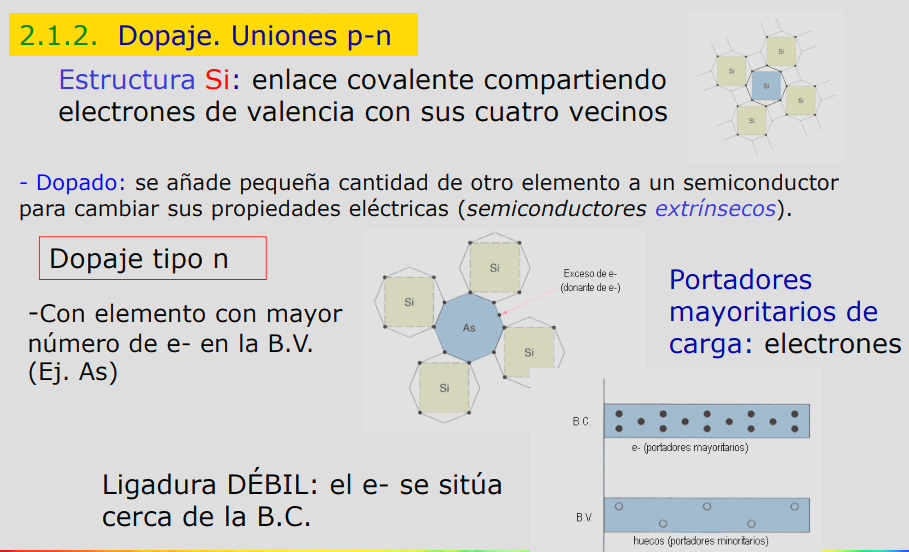
\includegraphics[width=0.7\textwidth]{IMG/led8.png}
	\end{figure}
	
	\esp
	
	En los compuestos dopados \textit{tipo p}, la estrategia es la contraria: sustituimos algunos de los átomos en este caso de $Si$ por otro elemento con menos electrones de valencia (por ejemplo, el $Al$, que tiene tres), con lo cual se crea un defecto de electrones en la red (uno de los cuatro vecinos del cada átomo de $Al$ no puede compartir electrones) y a este defecto se denomina \textit{hueco}. Los movimientos de electrones dentro del material pueden verse de forma equivalente como movimientos de huecos: cuando un electrón pasa a ocupar un hueco, el hueco cambia de posición a la anterior que ocupaba el electrón. Estos compuestos son potencialmente receptores de electrones, y tienden a cargarse negativamente. Los portadores mayoritarios de carga serían en este caso los huecos, según lo hemos explicado.
	
	\esp
	
	La proporción de dopante suele ser de 100-1000 átomos por cada millón de átomos de compuesto puro. Se notan con dos puntos tras el compuesto puro y a continuación el elemento dopante. Por ejemplo, $GaAs:Ge$ (arseniuro de galio dopado con germanio), o $Ge:B$ (germanio dopado con boro).
	
	\esp
	
	Las \textit{uniones p-n} son uno de los dispositivos más útiles y eficaces en optoelectrónica. Se forman por contacto de un semiconductor dopado \textit{tipo p} con otro dopado de \textit{tipo n}, bien del mismo material puro con distinto dopante (\textit{homounión}), o de distintos materiales semiconductores (\textit{heterounión}). En la figura 3, podemos ver esquemas de materiales de ambos tipos, y cómo la distribución de niveles (bandas) del \textit{tipo n} está a un nivel de energía diferente que en el \textit{tipo p}.
	
	\esp
	
	En la figura 3, vemos representados los niveles de Fermi correspondientes a ambos materiales, que muestran cómo los electrones del \textit{tipo n} se sitúan un poco por debajo de la B.C. y los del \textit{tipo p} un poco por encima de la B.V. El nivel de Fermi se define como el nivel energético para el cual, examinando la distribución de los electrones de un material en los diferentes niveles de energía, encontraríamos un 50 por ciento de la población en niveles superiores y el restante 50 por ciento en niveles inferiores. Dado que los electrones del semiconductor dopado \textit{tipo n} están más cerca de la banda de conducción, su nivel de Fermi es superior al del material dopado \textit{tipo p}, que tiene bastantes menos electrones en dicha banda. Al poner en contacto mediante una unión metalúrgica o cristalina el material \textit{tipo p} con el \textit{tipo n}, se produce un doblado de las bandas debido a la necesidad de continuidad en el material y a la diferencia de niveles energéticos que hemos esquematizado. También se crea una barrera de potencial, proceso que vamos a ver un poco más despacio. Como resultado de este proceso, el lado \textit{tipo p} próximo...

	\printbibliography[title={Bibliografía}]
\end{document}